\documentclass[10pt,twocolumn,letterpaper]{article}

% If cvpr.sty is available in your local template folder, keep this line.
% Otherwise, replace with your course-provided CVPR template settings.
\usepackage{cvpr}
\usepackage{times}
\usepackage{epsfig}
\usepackage{graphicx}
\usepackage{amsmath}
\usepackage{amssymb}
\usepackage{booktabs}
\usepackage{multirow}
\usepackage{xcolor}
\usepackage{url}
\usepackage[hidelinks]{hyperref}
\usepackage{tikz}
\usetikzlibrary{arrows.meta,positioning,shapes.geometric}

\cvprfinalcopy % CAMERA-READY version
\def\cvprPaperID{0000}
\def\confName{CVPR}
\def\confYear{2026}

\title{Video Object Removal and Background Restoration:\
From Hand-crafted Baselines to Quality-Gated Refinement}

\author{Group 16: Yuqi Ren, Anyi Wang\\
\url{https://github.com/mathway18/CV_project}}

\begin{document}
\maketitle

\begin{abstract}
We study video object removal and background restoration under a three-stage course setting: (1) a hand-crafted baseline with detection, motion filtering, and classical inpainting; (2) an AI-driven pipeline combining SAM 2 and ProPainter; and (3) a quality-gated extension that performs keyframe repair and frame-level fallback for stability. Our implementation emphasizes practical reproducibility, supports mandatory datasets (wild corridor, \textit{bmx-trees}, \textit{tennis}), and reports no-reference boundary seam and temporal warp metrics for Part 2 vs. Part 3. Experiments show that quality-gated refinement improves seam and temporal consistency on \textit{bmx-trees} and \textit{tennis}, while correctly preserving an already strong Part 2 output on the corridor sequence by rejecting harmful edits. This demonstrates that adaptive acceptance is more reliable than unconditional refinement in real-world video restoration. GitHub repository: \url{https://github.com/mathway18/CV_project}.
\end{abstract}

\section{Introduction}
Removing dynamic objects from videos and restoring plausible clean backgrounds is a representative problem in computer vision with applications in post-production, robotics, autonomous perception, and visual content editing. The problem is challenging because high-quality results require both accurate object localization over time and temporally coherent filling of large occluded regions.

Our project follows a progressive roadmap. In Part 1, we implement a hand-crafted baseline using YOLO-based segmentation, Lucas--Kanade optical flow filtering, mask dilation, and temporal-first restoration with OpenCV inpainting fallback. In Part 2, we reproduce a modern AI-driven strategy: SAM 2 for dynamic masks and ProPainter for video inpainting. In Part 3, we extend the system with quality-gated keyframe refinement, where candidate repaired frames are accepted only if local no-reference checks indicate improvement.

Our key contributions are:
\begin{itemize}
    \item A complete end-to-end implementation spanning traditional and modern pipelines for video object removal.
    \item A practical quality-gated refinement mechanism that avoids over-editing and preserves stable outputs.
    \item Quantitative and qualitative analysis across all mandatory datasets, including accepted/rejected refinement statistics.
\end{itemize}

\section{Related Work}
\subsection{Object Detection and Segmentation Foundations}
R-CNN~\cite{girshick2014rcnn} and Mask R-CNN~\cite{he2017maskrcnn} established two-stage detection/instance segmentation, while YOLO~\cite{redmon2016yolo} provided a strong real-time one-stage alternative. DETR~\cite{carion2020detr} introduced transformer-based end-to-end detection. Segment Anything (SAM)~\cite{kirillov2023sam} generalized promptable segmentation, and SAM 2~\cite{ravi2024sam2} extended this capability to video settings.

\subsection{Video Object Tracking and Dynamic Segmentation}
Track-Anything~\cite{yang2023trackanything} combines SAM-style segmentation with temporal tracking for interactive video object extraction. Recent geometry-centric methods such as VGGT4D~\cite{hu2025vggt4d}, built on visual geometry transformers~\cite{wang2025vggt}, show another route to dynamic cue mining. Newer foundation-model directions (SAM 3~\cite{carion2025sam3}, MapAnything~\cite{keetha2025mapanything}, Pi3~\cite{wang2025pi3}) suggest that richer 3D/4D priors may further improve video masks.

\subsection{Video Inpainting and Generative Restoration}
Classical flow-guided completion FGVC~\cite{gao2020fgvc} and end-to-end E2FGVI~\cite{li2022e2fgvi} advanced temporal inpainting quality. ProPainter~\cite{zhou2023propainter} combines dual-domain propagation and sparse transformers to handle large occlusions robustly and serves as our Part 2 core inpainting engine. For hard cases where background content never appears in the sequence, latent diffusion~\cite{rombach2022ldm} with controllable conditioning (e.g., ControlNet~\cite{zhang2023controlnet}) provides a promising generative fallback.

\section{Method}
\subsection{Overall Roadmap}
Figure~\ref{fig:pipeline} summarizes the full pipeline. Given an input video, we first generate dynamic-object masks (Part 1: YOLO + motion filter; Part 2: YOLO prompts + SAM 2). We then restore masked regions (Part 1: temporal borrowing + OpenCV inpainting; Part 2: ProPainter). Finally, Part 3 optionally refines keyframes and uses quality-gated fallback to preserve stability.

\begin{figure}[t]
\centering
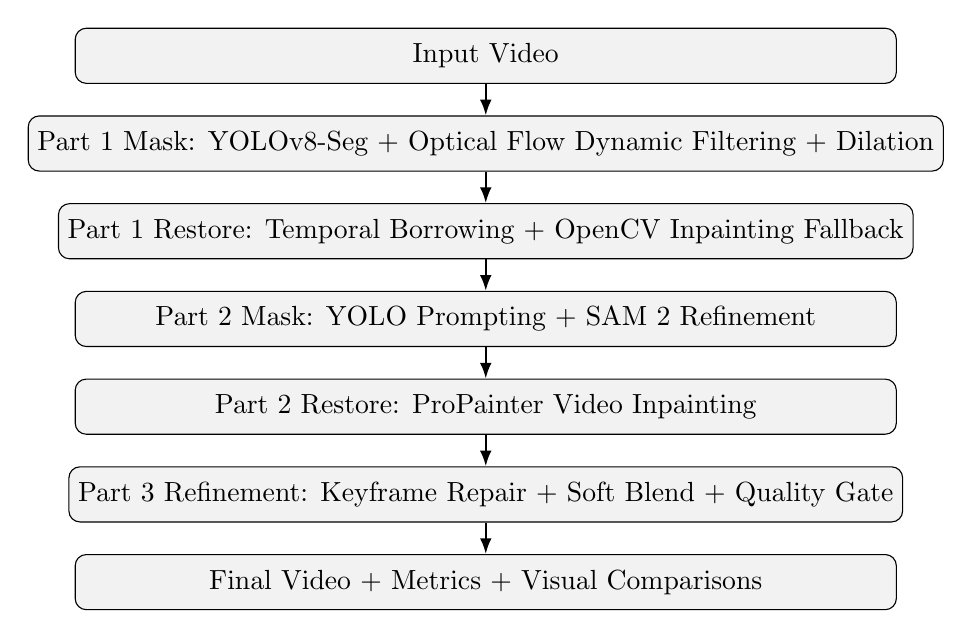
\begin{tikzpicture}[
    node distance=4mm and 3mm,
    block/.style={draw, rounded corners, align=center, minimum width=0.86\linewidth, minimum height=7mm, fill=gray!10},
    arr/.style={-{Latex[length=2mm]}, thick}
]
\node[block] (in) {Input Video};
\node[block, below=of in] (m1) {Part 1 Mask: YOLOv8-Seg + Optical Flow Dynamic Filtering + Dilation};
\node[block, below=of m1] (i1) {Part 1 Restore: Temporal Borrowing + OpenCV Inpainting Fallback};
\node[block, below=of i1] (m2) {Part 2 Mask: YOLO Prompting + SAM 2 Refinement};
\node[block, below=of m2] (i2) {Part 2 Restore: ProPainter Video Inpainting};
\node[block, below=of i2] (p3) {Part 3 Refinement: Keyframe Repair + Soft Blend + Quality Gate};
\node[block, below=of p3] (out) {Final Video + Metrics + Visual Comparisons};
\draw[arr] (in) -- (m1);
\draw[arr] (m1) -- (i1);
\draw[arr] (i1) -- (m2);
\draw[arr] (m2) -- (i2);
\draw[arr] (i2) -- (p3);
\draw[arr] (p3) -- (out);
\end{tikzpicture}
\caption{Technical roadmap from baseline to AI-driven restoration and quality-gated extension.}
\label{fig:pipeline}
\end{figure}

\subsection{Part 1: Hand-crafted Baseline}
\textbf{Dynamic mask extraction.}
We detect target categories and estimate object-wise motion magnitude using sparse optical flow on internal feature points. Static instances are filtered out, and binary masks are dilated to cover object boundaries and motion blur.

\textbf{Background restoration.}
For each masked pixel, we prioritize temporal borrowing from neighboring frames at identical spatial locations, then apply classical inpainting when temporal evidence is unavailable. This design is lightweight and easy to reproduce, but tends to blur highly textured or large missing regions.

\subsection{Part 2: AI-driven Pipeline}
\textbf{SAM 2 mask refinement.}
We use detector cues as prompts and run SAM 2 for high-quality dynamic segmentation. Practical adjustments include restricting SAM 2 predictions with detector masks and disabling temporal stabilization by default when it propagates false positives.

\textbf{ProPainter inpainting.}
Frame-wise masks are passed to ProPainter, which leverages motion/feature propagation and sparse transformer modeling to produce temporally consistent restored videos.

\subsection{Part 3: Quality-Gated Keyframe Refinement}
Part 3 introduces a conservative refinement strategy:
\begin{enumerate}
    \item Select keyframes with non-empty masks.
    \item Generate candidate repairs (OpenCV backend for reproducibility; optional diffusion backend for exploration).
    \item Softly blend repaired content into Part 2 outputs.
    \item Accept the candidate only if local no-reference checks improve seam/temporal behavior and satisfy regression thresholds; otherwise fall back to Part 2.
\end{enumerate}
Unlike unconditional post-processing, this stage is explicitly formulated as a \emph{decision problem}. For each candidate frame $I_t^{(3)}$ and baseline frame $I_t^{(2)}$, we evaluate local boundary seam, temporal warp consistency, and masked-region change magnitude. A frame is accepted only when (i) seam does not regress, (ii) temporal error does not exceed a configured regression bound, and (iii) masked-region drift remains under a safety threshold. Otherwise, we directly copy $I_t^{(2)}$ to the final output. This design makes Part 3 robust in two opposite regimes: it can improve difficult sequences (large texture/occlusion) while preserving strong Part 2 outputs in easy or already-clean sequences.

\section{Experiments}
\subsection{Experimental Setup}
We evaluate all mandatory videos: \textit{bmx-trees} (80 frames, $432\times240$), \textit{tennis} (70 frames, $432\times240$), and wild corridor (192 frames, $1280\times720$). Part 2 is the fixed baseline (SAM 2 + ProPainter). Part 3 is the quality-gated keyframe refinement stage built on top of those outputs.

\subsection{Metrics}
Because clean ground-truth videos are unavailable for these mandatory sequences, we use no-reference diagnostics:
\begin{itemize}
    \item \textbf{Boundary seam score} (lower is better): discontinuity around mask boundaries.
    \item \textbf{Temporal warp error} (lower is better): frame-to-frame inconsistency after motion warping.
    \item \textbf{Masked texture statistic} (diagnostic): local high-frequency content in masked regions.
    \item \textbf{Gate acceptance behavior}: accepted/rejected frames and acceptance rate.
\end{itemize}
These metrics are computed from saved outputs in \texttt{outputs/part3\_*\allowbreak/part3\_eval.json} and summarized in \texttt{outputs/part3\_metrics\_summary.json}.

\subsection{Main Quantitative Results}
\begin{table}[t]
\centering
\scriptsize
\caption{Part 2 vs. Part 3 quantitative comparison. Seam and warp are lower-is-better.}
\label{tab:main}
\begin{tabular}{lrrrrrr}
\toprule
Dataset & P2 Seam & P3 Seam & $\Delta$Seam\% & P2 Warp & P3 Warp & $\Delta$Warp\% \\
\midrule
bmx-trees & 18.2920 & \textbf{18.1038} & +1.03 & 5.3090 & \textbf{5.1043} & +3.86 \\
tennis & 3.7167 & \textbf{3.5840} & +3.57 & 2.1920 & \textbf{2.1745} & +0.80 \\
wild corridor & 3.1025 & 3.1025 & 0.00 & 1.4674 & 1.4674 & 0.00 \\
\bottomrule
\end{tabular}
\end{table}

\begin{table}[t]
\centering
\scriptsize
\caption{Gate behavior and masked-region diagnostics.}
\label{tab:gate}
\begin{tabular}{lrrrrrr}
\toprule
Dataset & Frames & Acc. & Rej. & Acc.\% & Mask px & Texture $\Delta$\% \\
\midrule
bmx-trees & 80 & 15 & 65 & 18.75 & 3142.7 & -7.21 \\
tennis & 70 & 53 & 17 & 75.71 & 12688.8 & -20.98 \\
wild corridor & 192 & 0 & 192 & 0.00 & 58460.6 & 0.00 \\
\bottomrule
\end{tabular}
\end{table}

Table~\ref{tab:main} shows that Part 3 improves both seam and temporal consistency on \textit{bmx-trees} and \textit{tennis}, while preserving wild corridor unchanged. Table~\ref{tab:gate} reveals that this behavior is tightly linked to gate decisions: the gate is highly selective on \textit{bmx-trees} (18.75\% acceptance), permissive on \textit{tennis} (75.71\%), and fully rejecting on corridor (0\%). This confirms that the refinement stage functions as an adaptive controller rather than a fixed transformation.

\subsection{Per-Dataset Analysis}
\textbf{\textit{bmx-trees}.} This sequence has challenging high-frequency background content (trees/branches), where seam artifacts are easy to introduce. The gate accepts only 15/80 frames, but this small subset is sufficient to yield measurable gains: seam improves by 1.03\% and temporal warp by 3.86\%. The relatively low acceptance rate indicates that many candidate edits are risky in this scene; selective acceptance prevents quality collapse.

\textbf{\textit{tennis}.} This sequence admits many stable corrections (53/70 accepted). Seam improves by 3.57\% and temporal warp by 0.80\%, showing that accepted edits are mostly safe and useful. The larger texture drop suggests stronger smoothing in masked regions; however, the boundary and temporal metrics still improve, indicating a favorable trade-off for this dataset.

\textbf{Wild corridor.} All 192 candidate frames are rejected, and Part 3 exactly matches Part 2. This is not a failure; it is intended behavior of quality-gated refinement when the baseline is already strong and additional edits are likely to be harmful. The gate therefore acts as a safety mechanism that protects an already good restoration.

\subsection{Qualitative Comparison}
\begin{figure*}[t]
\centering
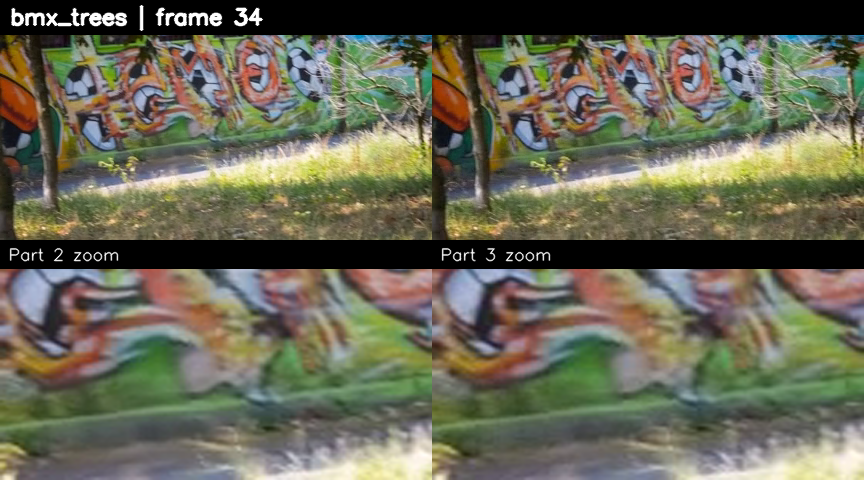
\includegraphics[width=0.32\textwidth]{report_assets/bmx_trees_compare.png}\hfill
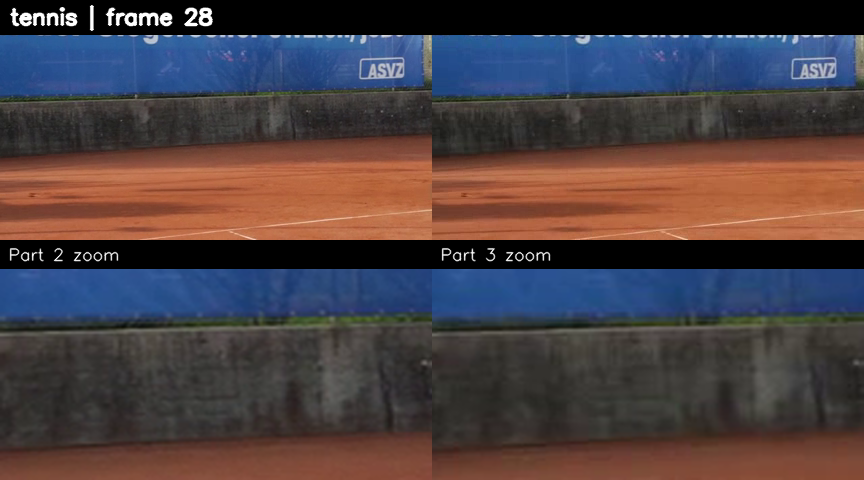
\includegraphics[width=0.32\textwidth]{report_assets/tennis_compare.png}\hfill
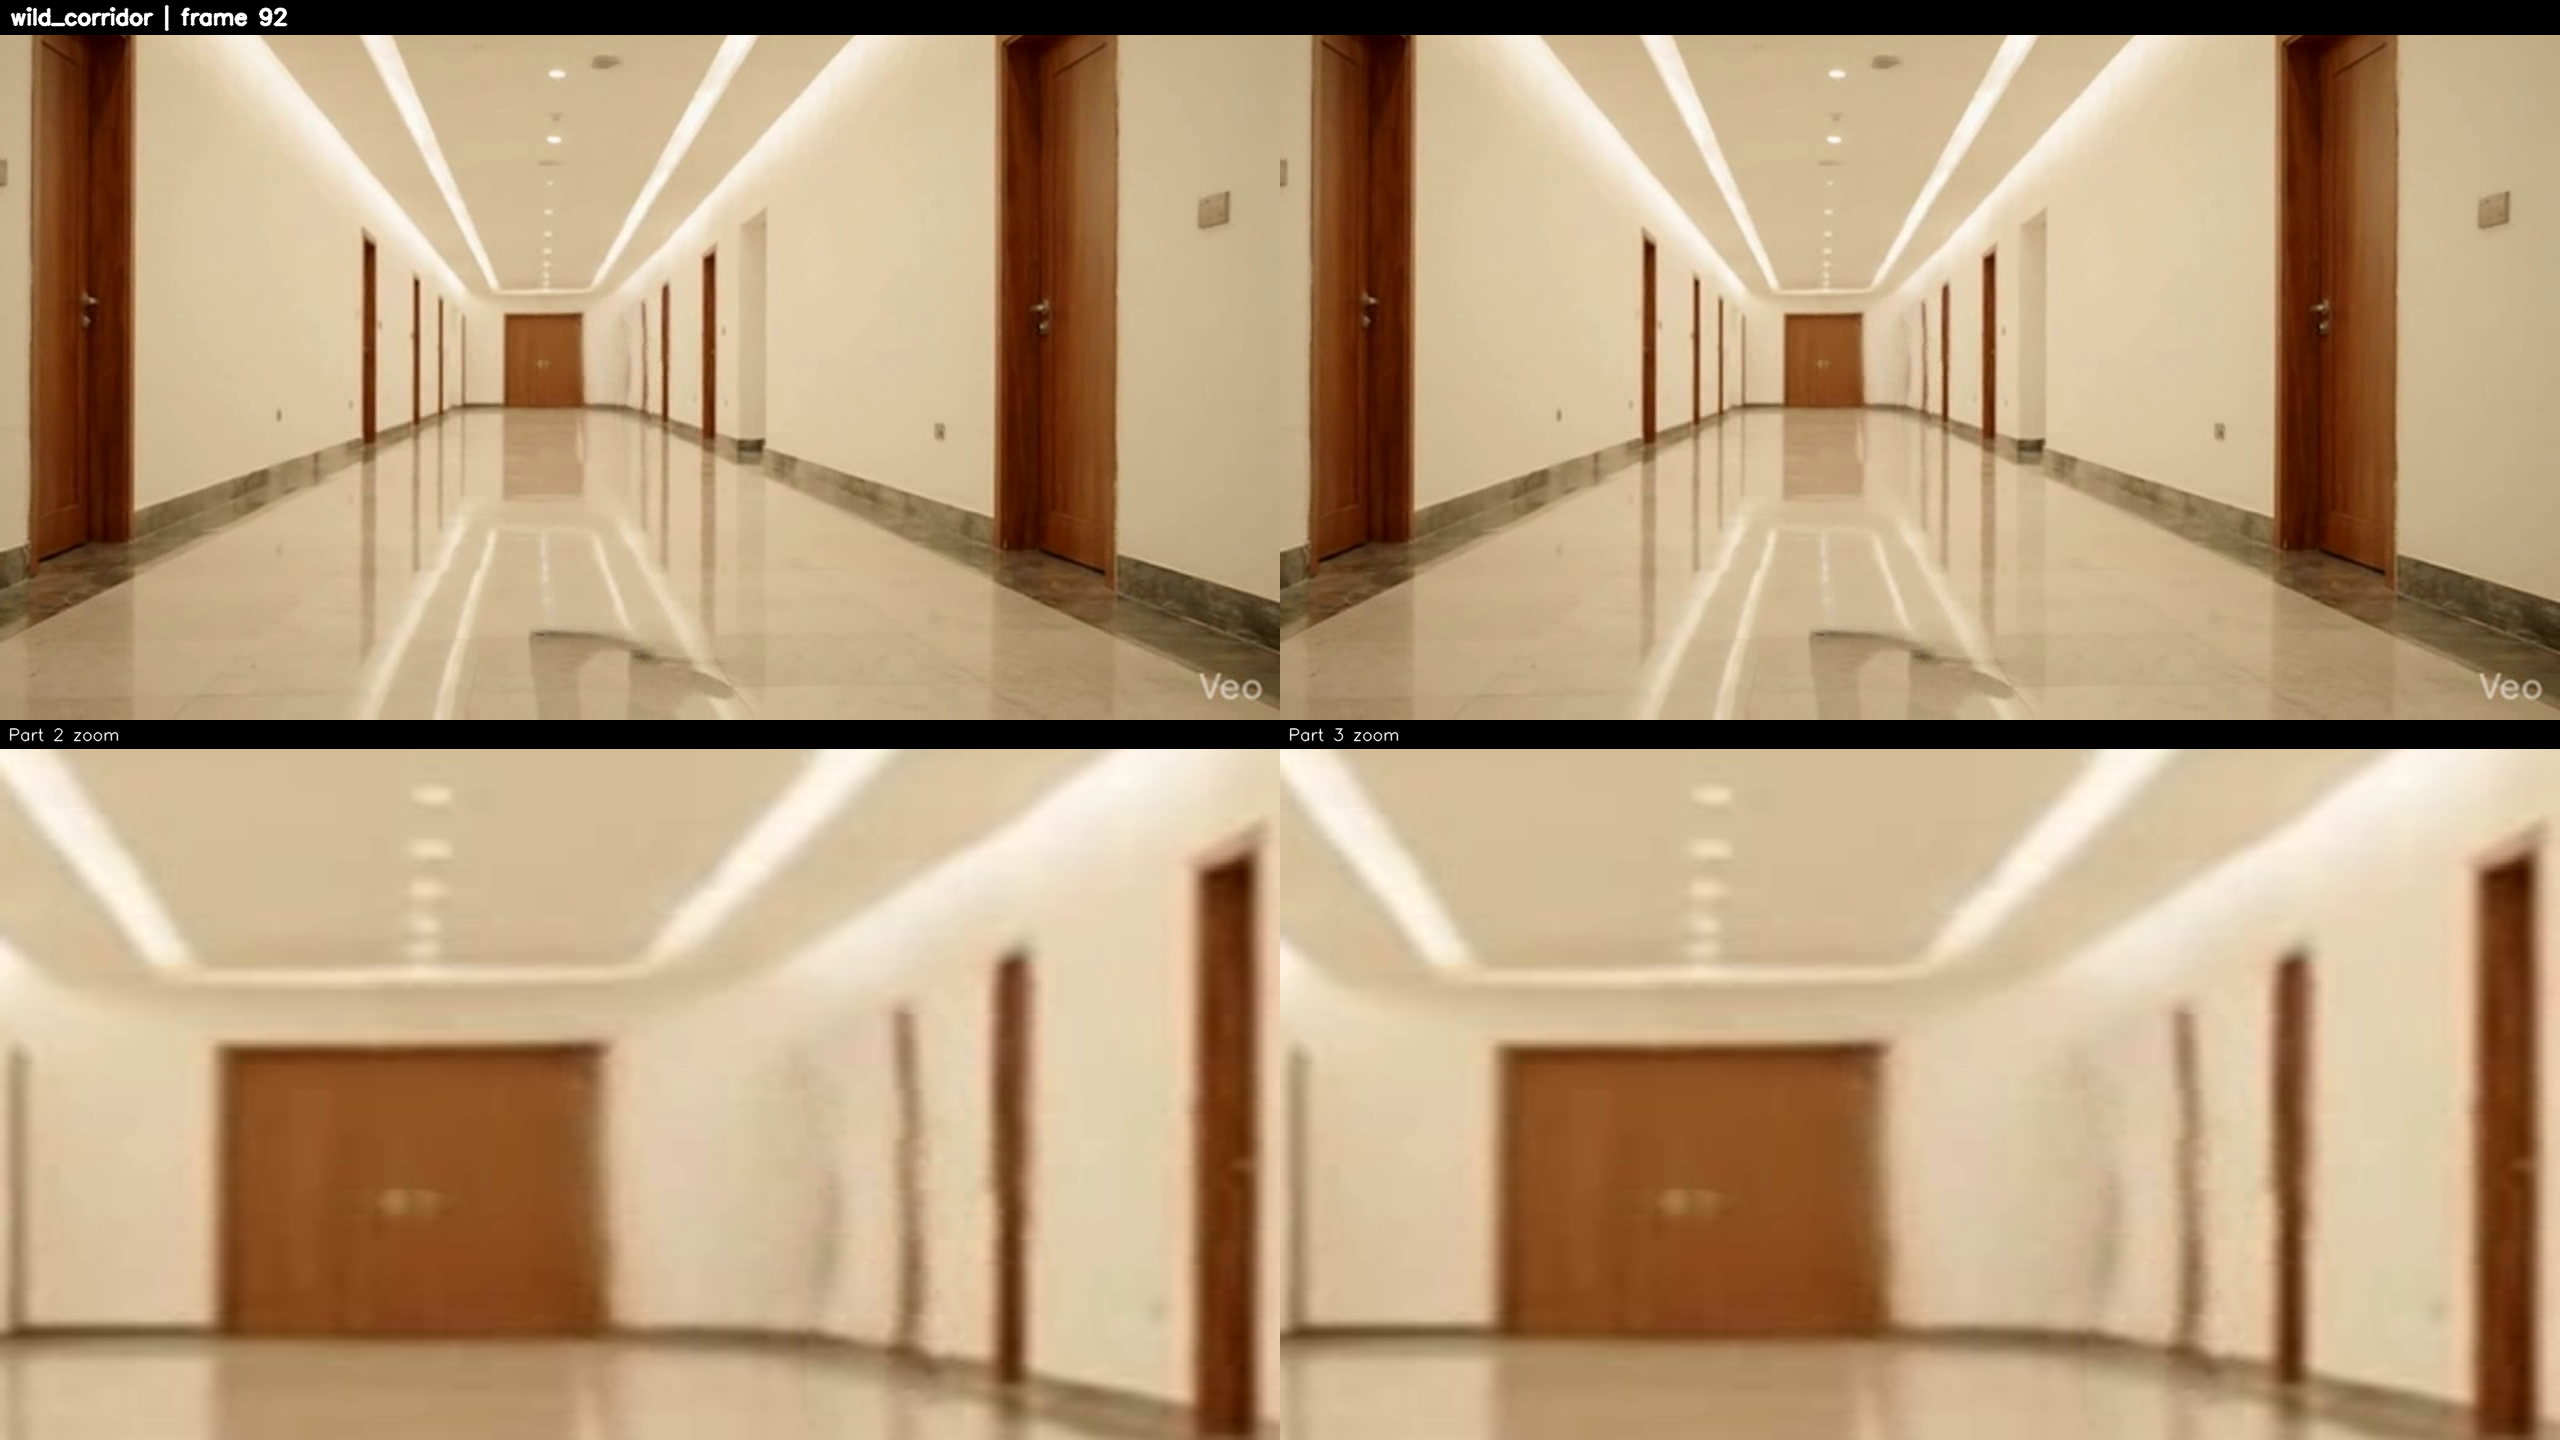
\includegraphics[width=0.32\textwidth]{report_assets/wild_corridor_compare.png}
\caption{Real frame-level qualitative comparisons extracted from final outputs. Each panel contains Part 2 frame, Part 3 frame, and corresponding zoomed views (same timestamp). \textit{bmx-trees} and \textit{tennis} show cleaner transitions around removal regions; wild corridor remains visually equivalent due to full gate rejection.}
\label{fig:qual-main}
\end{figure*}

\begin{figure}[t]
\centering
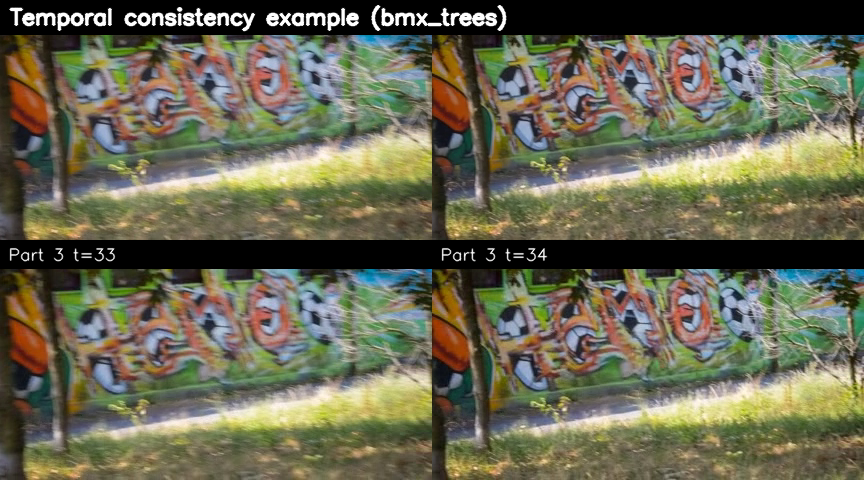
\includegraphics[width=\linewidth]{report_assets/bmx_temporal.png}
\caption{Temporal consistency example on \textit{bmx-trees} (two adjacent frames). Part 3 reduces flicker-like boundary variation while preserving frame continuity.}
\label{fig:qual-temporal}
\end{figure}

\subsection{Failure Modes and Trade-offs}
The results also expose meaningful trade-offs. First, no-reference metrics may not fully capture perceptual realism, especially in large uniform regions where seam reduction can coincide with over-smoothing. Second, datasets have different spatial resolutions (e.g., corridor at $1280\times720$ vs. others at $432\times240$), so absolute metric magnitudes are not directly interchangeable across datasets; trends within each dataset are more reliable than cross-dataset raw-value ranking. Third, masked texture can decrease even when seam/warp improve, so final judgment should combine quantitative diagnostics with visual inspection (Figure~\ref{fig:qual-main}).

\subsection{Discussion}
Overall, the experiments support a practical lesson for video restoration: \emph{refinement should be conditional}. A global always-on refinement step is brittle, while quality gating enables dataset-specific adaptation. In difficult scenes, selective accepted edits improve quality; in already-clean scenes, conservative rejection prevents regressions. This is particularly important in production workflows where failure cases are more costly than modest missed gains.

\section{Conclusion}
We presented a complete video object removal project that progresses from classical computer-vision baselines to modern foundation-model-based restoration and an adaptive Part 3 extension. With mandatory datasets, the final system demonstrates two complementary strengths: (1) measurable improvement where refinement is beneficial (\textit{bmx-trees}, \textit{tennis}), and (2) safe non-intervention where the baseline is already near-optimal (wild corridor).

\textbf{Limitations.}
Our quantitative analysis for mandatory data is no-reference and therefore indirect. The diffusion backend is optional and not always feasible in limited hardware settings. Detector/SAM failures may still propagate into inpainting, and no-reference diagnostics cannot perfectly reflect perceptual naturalness under all texture regimes.

\textbf{Future Work.}
Future directions include: (1) larger-scale evaluation on benchmarks with ground truth (IoU/PSNR/SSIM + user study); (2) stronger video foundation models for dynamic mask quality; and (3) learning-based acceptance policies that jointly optimize seam, temporal stability, and texture retention rather than relying on manually tuned thresholds.

\begin{thebibliography}{17}\small

\bibitem{carion2025sam3}
Nicolas Carion, Laura Gustafson, Yuan-Ting Hu, Shoubhik Debnath, Ronghang Hu, Didac Suris, Chaitanya Ryali, Kalyan Vasudev Alwala, Haitham Khedr, Andrew Huang, et al.
SAM 3: Segment anything with concepts.
\textit{arXiv preprint arXiv:2511.16719}, 2025.

\bibitem{carion2020detr}
Nicolas Carion, Francisco Massa, Gabriel Synnaeve, Nicolas Usunier, Alexander Kirillov, and Sergey Zagoruyko.
End-to-end object detection with transformers.
In \textit{European Conference on Computer Vision}, 2020.

\bibitem{gao2020fgvc}
Chen Gao, Ayush Saraf, Jia-Bin Huang, and Johannes Kopf.
Flow-Guided Video Completion.
In \textit{European Conference on Computer Vision}, 2020.

\bibitem{girshick2014rcnn}
Ross Girshick, Jeff Donahue, Trevor Darrell, and Jitendra Malik.
Rich feature hierarchies for accurate object detection and semantic segmentation.
In \textit{CVPR}, 2014.

\bibitem{he2017maskrcnn}
Kaiming He, Georgia Gkioxari, Piotr Doll{\'a}r, and Ross Girshick.
Mask R-CNN.
In \textit{ICCV}, 2017.

\bibitem{hu2025vggt4d}
Yu Hu, Chong Cheng, Sicheng Yu, Xiaoyang Guo, and Hao Wang.
VGGT4D: Mining motion cues in visual geometry transformers for 4D scene reconstruction.
\textit{arXiv preprint arXiv:2511.19971}, 2025.

\bibitem{keetha2025mapanything}
Nikhil Keetha, Norman Muller, Johannes Schonberger, Lorenzo Porzi, Yuchen Zhang, Tobias Fischer, Arno Knapitsch, Duncan Zauss, Ethan Weber, Nelson Antunes, et al.
MapAnything: Universal feed-forward metric 3D reconstruction.
\textit{arXiv preprint arXiv:2509.13414}, 2025.

\bibitem{kirillov2023sam}
Alexander Kirillov, Eric Mintun, Nikhila Ravi, Hanzi Mao, Chloe Rolland, Laura Gustafson, Tete Xiao, Spencer Whitehead, Alexander C. Berg, Wan-Yen Lo, et al.
Segment Anything.
In \textit{ICCV}, 2023.

\bibitem{li2022e2fgvi}
Zhen Li, Cheng-Ze Lu, Jianhua Qin, Chun-Le Guo, and Ming-Ming Cheng.
Towards an end-to-end framework for flow-guided video inpainting.
In \textit{CVPR}, 2022.

\bibitem{ravi2024sam2}
Nikhila Ravi, Valentin Gabeur, Yuan-Ting Hu, Ronghang Hu, Chaitanya Ryali, Tengyu Ma, Haitham Khedr, Roman R\"adle, Chloe Rolland, Laura Gustafson, et al.
SAM 2: Segment anything in images and videos.
\textit{arXiv preprint arXiv:2408.00714}, 2024.

\bibitem{redmon2016yolo}
Joseph Redmon, Santosh Divvala, Ross Girshick, and Ali Farhadi.
You only look once: Unified, real-time object detection.
In \textit{CVPR}, 2016.

\bibitem{rombach2022ldm}
Robin Rombach, Andreas Blattmann, Dominik Lorenz, Patrick Esser, and Bj\"orn Ommer.
High-resolution image synthesis with latent diffusion models.
In \textit{CVPR}, 2022.

\bibitem{wang2025vggt}
Jianyuan Wang, Minghao Chen, Nikita Karaev, Andrea Vedaldi, Christian Rupprecht, and David Novotny.
VGGT: Visual geometry grounded transformer.
In \textit{CVPR}, 2025.

\bibitem{wang2025pi3}
Yifan Wang, Jianjun Zhou, Haoyi Zhu, Wenzheng Chang, Yang Zhou, Zizun Li, Junyi Chen, Jiangmiao Pang, Chunhua Shen, and Tong He.
Pi3: Permutation-equivariant visual geometry learning.
\textit{arXiv preprint arXiv:2507.13347}, 2025.

\bibitem{yang2023trackanything}
Jinyu Yang, Mingqi Gao, Zhe Li, Shang Gao, Fangjing Wang, and Feng Zheng.
Track Anything: Segment anything meets videos.
\textit{arXiv preprint arXiv:2304.11968}, 2023.

\bibitem{zhang2023controlnet}
Lvmin Zhang, Anyi Rao, and Maneesh Agrawala.
Adding conditional control to text-to-image diffusion models.
In \textit{ICCV}, 2023.

\bibitem{zhou2023propainter}
Shangchen Zhou, Chongyi Li, Kelvin C. K. Chan, and Chen Change Loy.
ProPainter: Improving propagation and transformer for video inpainting.
In \textit{ICCV}, 2023.

\end{thebibliography}

\end{document}
